% Standalone non-technical overview of SwegHammer.
% Build: pdflatex OVERVIEW.tex
% Produces a single-page PDF of just the diagram, suitable for sharing.

\documentclass[border=12pt]{standalone}

\usepackage[T1]{fontenc}
\usepackage{lmodern}
\usepackage{xcolor}
\usepackage{tikz}
\usetikzlibrary{arrows.meta, positioning, calc}

\definecolor{simblue}{HTML}{1F6FB2}
\definecolor{realorange}{HTML}{D2691E}
\definecolor{greentick}{HTML}{2E8B57}
\definecolor{greytext}{HTML}{555555}

\begin{document}
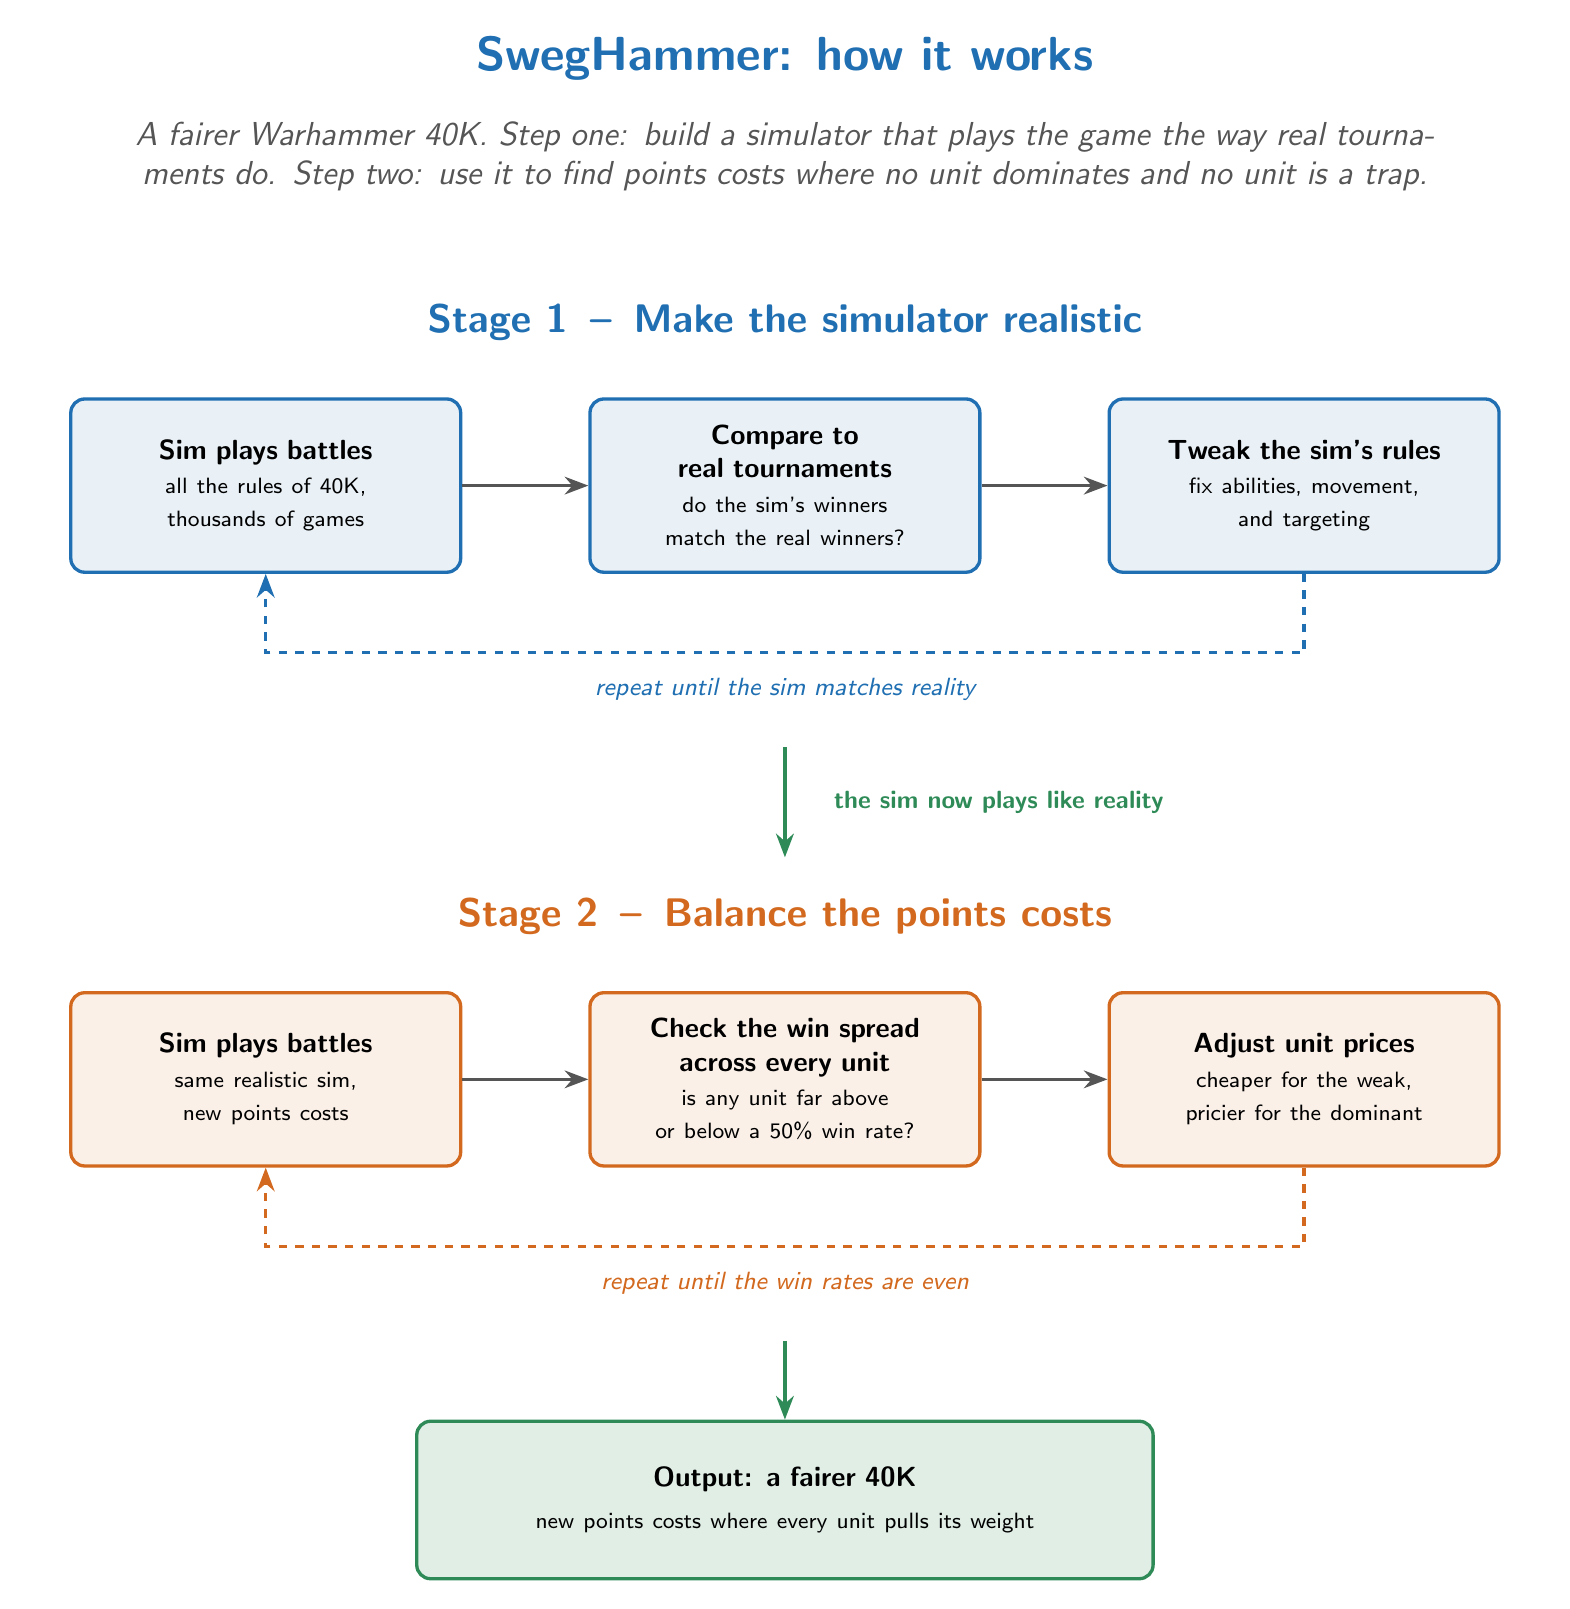
\begin{tikzpicture}[
    >={Stealth[length=3mm]},
    node distance=14mm and 16mm,
    every node/.style={font=\sffamily},
    title/.style={font=\sffamily\LARGE\bfseries, text=simblue, align=center},
    oneliner/.style={
      font=\sffamily\large\itshape, text=greytext,
      align=center, text width=190mm
    },
    stageheader/.style={font=\sffamily\bfseries\Large, align=center},
    bluebox/.style={
      rectangle, rounded corners=5pt, draw=simblue, very thick,
      fill=simblue!10, text width=46mm, align=center,
      minimum height=22mm, inner sep=5pt
    },
    orangebox/.style={
      rectangle, rounded corners=5pt, draw=realorange, very thick,
      fill=realorange!10, text width=46mm, align=center,
      minimum height=22mm, inner sep=5pt
    },
    goalbox/.style={
      rectangle, rounded corners=5pt, draw=greentick, very thick,
      fill=greentick!15, text width=90mm, align=center,
      minimum height=20mm, inner sep=5pt
    },
    arrow/.style={->, very thick, draw=greytext},
    loopblue/.style={->, very thick, draw=simblue, dashed},
    looporange/.style={->, very thick, draw=realorange, dashed},
    bridge/.style={->, ultra thick, draw=greentick},
    arrowlabel/.style={font=\sffamily\small\itshape, align=center},
    bridgelabel/.style={font=\sffamily\small\bfseries, text=greentick, align=center}
  ]

  % ===== header =====
  \node[title] (heading) {SwegHammer: how it works};
  \node[oneliner, below=3mm of heading] (oneliner) {%
    A fairer Warhammer 40K. Step one: build a simulator that plays
    the game the way real tournaments do. Step two: use it to find
    points costs where no unit dominates and no unit is a trap.%
  };

  % ===== Stage 1 — middle box centered under header =====
  \node[stageheader, text=simblue, below=12mm of oneliner] (h1)
    {Stage 1 \,--\, Make the simulator realistic};

  \node[bluebox, below=6mm of h1] (real)
    {\textbf{Compare to}\\\textbf{real tournaments}\\[3pt]
     \footnotesize do the sim's winners\\match the real winners?};
  \node[bluebox, left=of real] (sim1)
    {\textbf{Sim plays battles}\\[3pt]
     \footnotesize all the rules of 40K,\\thousands of games};
  \node[bluebox, right=of real] (tweaksim)
    {\textbf{Tweak the sim's rules}\\[3pt]
     \footnotesize fix abilities, movement,\\and targeting};

  \draw[arrow] (sim1) -- (real);
  \draw[arrow] (real) -- (tweaksim);
  \draw[loopblue] (tweaksim.south) -- ++(0,-10mm) -| (sim1.south);
  \node[arrowlabel, text=simblue, anchor=north]
    at ($(sim1.south)!0.5!(tweaksim.south)+(0,-12mm)$)
    {repeat until the sim matches reality};

  % ===== bridge: Stage 1 -> Stage 2 =====
  \coordinate (s1bottom) at ($(sim1.south)!0.5!(tweaksim.south)+(0,-22mm)$);
  \coordinate (s2top)    at ($(s1bottom)+(0,-14mm)$);

  \draw[bridge] (s1bottom) -- (s2top);
  \node[bridgelabel, anchor=west]
    at ($(s1bottom)!0.5!(s2top)+(5mm,0)$)
    {the sim now plays like reality};

  % ===== Stage 2 — same shape, orange =====
  \node[stageheader, text=realorange, below=4mm of s2top, anchor=north] (h2)
    {Stage 2 \,--\, Balance the points costs};

  \node[orangebox, below=6mm of h2] (spread)
    {\textbf{Check the win spread}\\\textbf{across every unit}\\[3pt]
     \footnotesize is any unit far above\\or below a 50\% win rate?};
  \node[orangebox, left=of spread] (sim2)
    {\textbf{Sim plays battles}\\[3pt]
     \footnotesize same realistic sim,\\new points costs};
  \node[orangebox, right=of spread] (tweakpts)
    {\textbf{Adjust unit prices}\\[3pt]
     \footnotesize cheaper for the weak,\\pricier for the dominant};

  \draw[arrow] (sim2) -- (spread);
  \draw[arrow] (spread) -- (tweakpts);
  \draw[looporange] (tweakpts.south) -- ++(0,-10mm) -| (sim2.south);
  \node[arrowlabel, text=realorange, anchor=north]
    at ($(sim2.south)!0.5!(tweakpts.south)+(0,-12mm)$)
    {repeat until the win rates are even};

  % ===== final output =====
  \coordinate (s2bottom) at ($(sim2.south)!0.5!(tweakpts.south)+(0,-22mm)$);
  \node[goalbox, below=10mm of s2bottom, anchor=north] (out)
    {\textbf{Output: a fairer 40K}\\[3pt]
     \footnotesize new points costs where every unit pulls its weight};
  \draw[bridge] (s2bottom) -- (out.north);

\end{tikzpicture}
\end{document}
